\section{Durchführung}

\subsection{Bau des Roboterarmes}
\schritt{1}{Den Roboterarm vorbereiten}{
Die Pappe schneidet ihr in sechs 30cm lange und 2cm breite Streifen.
Zwei davon werden auf 15cm gekürzt, zwei weitere auf 12cm.\\

Aus den Resten der gekürzten Streifen schneidet ihr zirka 12 kleine Pappquadrate.
Außerdem benötigt ihr vier Pappteile, die ihr wie auf dem Bild zuschneidet, und zwei Pappkreise, deren Durchmesser mit der Größe der Reifen übereinstimmt.\\
}


\schritt{2}{Den Roboterarm bauen}{
Die Pappstreifen werden jetzt zusammengeklebt.
Dafür klebt ihr die jeweils beiden gleichlangen Streifen mit Heißkleber zusammen, sodass ihr nun ein 30cm, ein 15cm und ein 12cm Pappstück habt.
Die vier Pappteile klebt ihr übereinander zu einem Klotz. An diesem können später die Stifte befestigt werden.\\
}


\subsection{Verbindung mit RaspberryPi}

\begin{center}
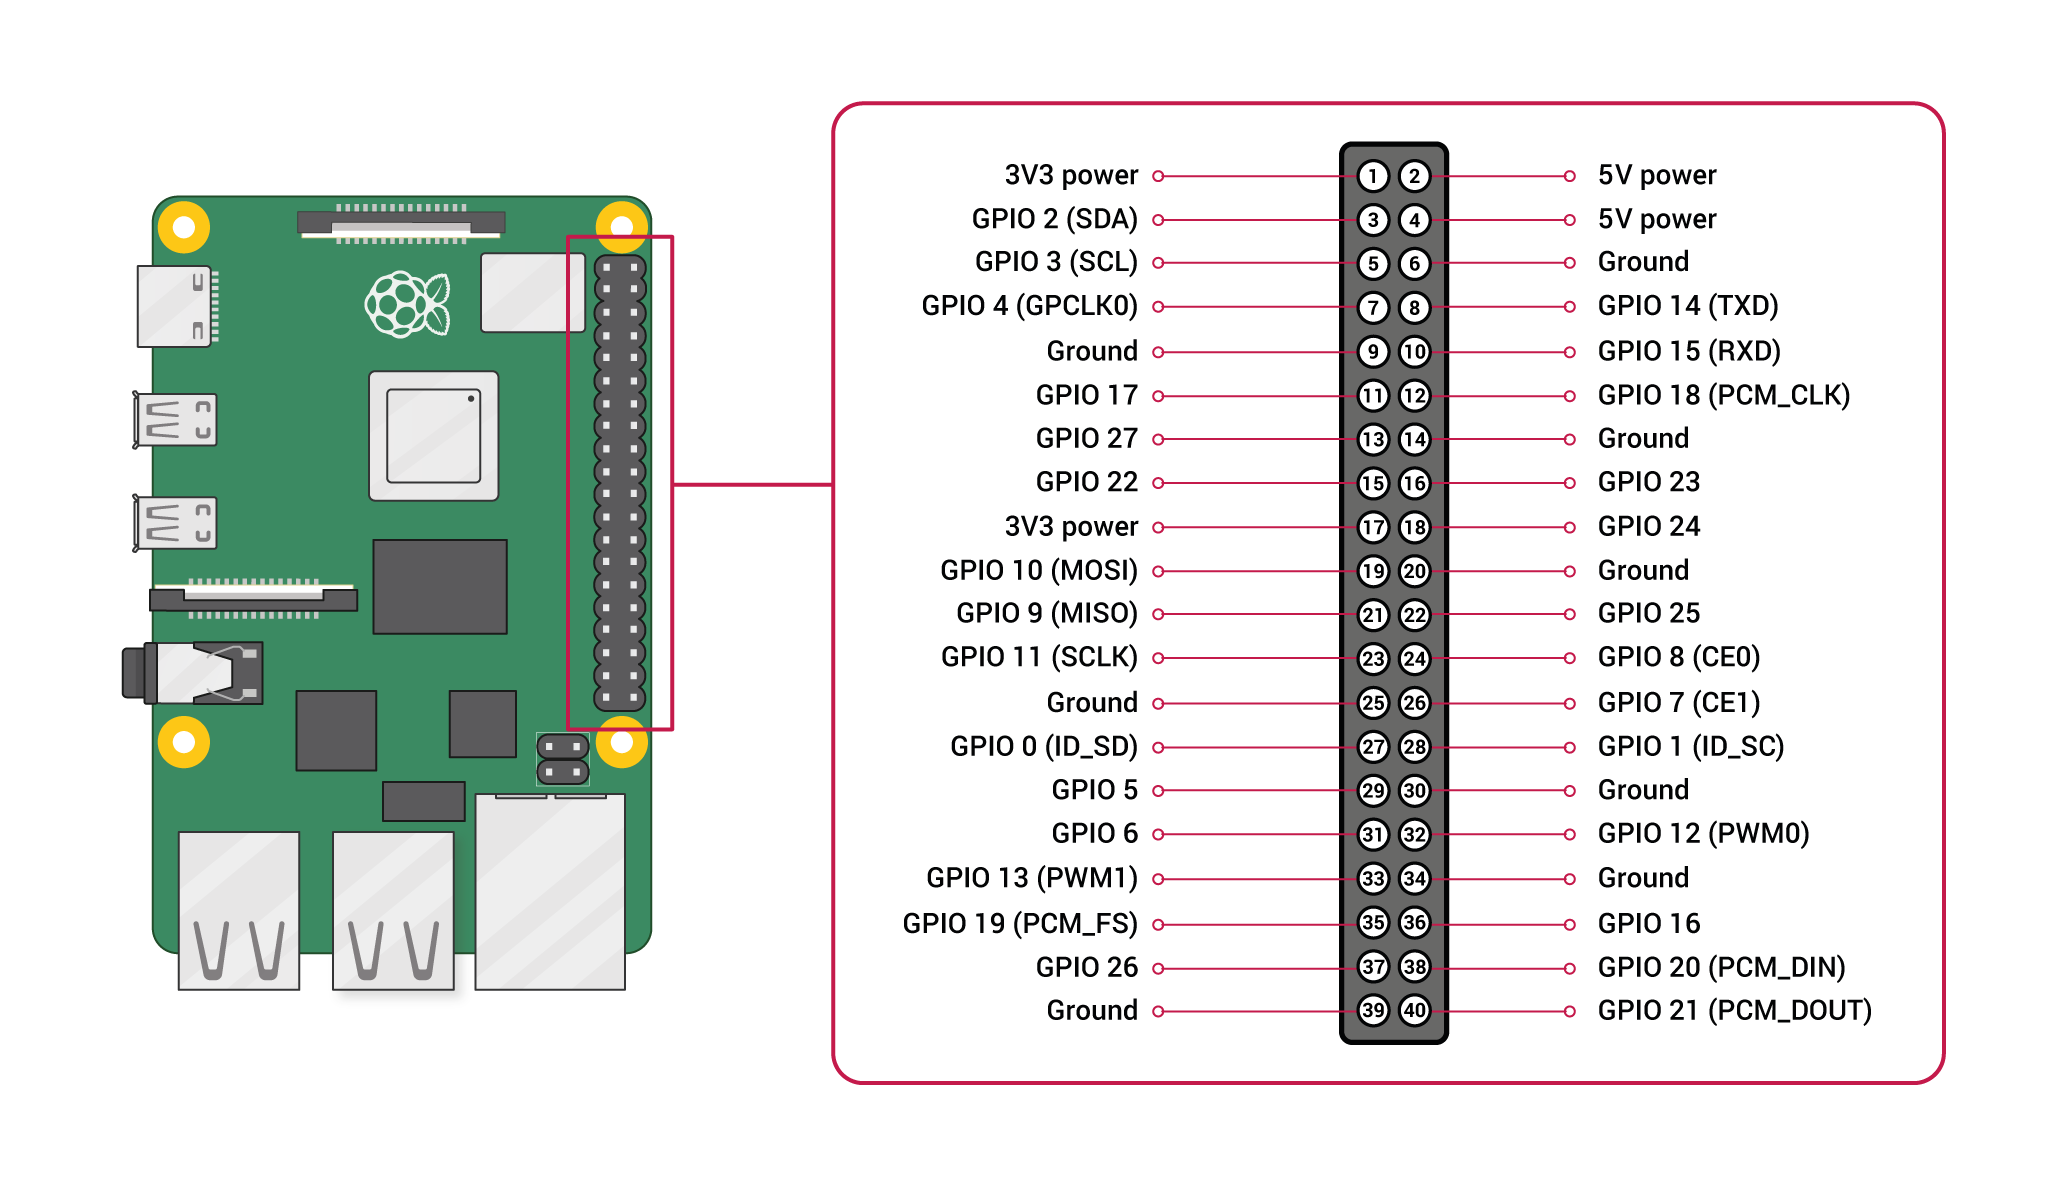
\includegraphics[width=\textwidth]{rpi_gpio_pinout.png}
\end{center}

\subsubsection{Verbindung Motor mit Treiber}
\subsubsection{Verbindung Treiber mit RaspberryPi}

\subsection{Programmierung}
\subsection{Programm A (Beispiel)}
\subsection{Programm B}
